%\documentclass[onecolumn,journal]{IEEEtran}
\documentclass[journal]{IEEEtran}
%\textwidth=14.6cm \textheight=22cm \headsep=1.0cm
%\oddsidemargin=.9cm \topmargin=-.6cm

% Proofreading purposes.
%\documentclass[12]{article}
%\renewcommand{\baselinestretch}{2}
%\oddsidemargin 0 in
%\textwidth 7.0 in

\usepackage{graphicx}
\usepackage{psfrag}
\usepackage{subfigure}

\begin{document}

\title{Power Allocation for OFDM-based Cooperative Relay Systems}

%\author{Victor~K.~Y.~Wu$^*$
%            and~Ye~(Geoffrey)~Li,~\IEEEmembership{Fellow,~IEEE}\\
%            School of Electrical and Computer Engineering \\
%            Georgia Institute of Technology \\
%            Atlanta, Georgia \\
%            Email: victor.wu@gatech.edu, liye@ece.gatech.edu
%\thanks{This work was supported by a research gift from the Nokia Research Center at Texas.}
%\thanks{*V. K. Y. Wu can be reached by telephone at (416) 512-6927 or by surface mail at 397 Ruth Avenue, North York, Ontario, Canada, M2M 2J1.}
%}

%\author{\authorblockN{Victor K. Y. Wu and Ye (Geoffrey) Li}
%\authorblockA{School of Electrical and Computer Engineering\\
%Georgia Institute of Technology\\
%Atlanta, Georgia\\
%Email: vwu3@ifp.uiuc.edu, liye@ece.gatech.edu} \and
%\authorblockN{Marilynn Green, Tony Reid, and Peter Wang}
%\authorblockA{Nokia Siemens Networks\\
%Dallas, Texas\\
%Email: \{marilynn.green, tony.reid, peter.wang\}@nsn.com} }

%\author{Victor~K.~Y.~Wu$^{\ast}$ \thanks{ \hspace*{-0.5cm} $\overline{~~~~~ \ast \mbox{The corresponding author }}$can be reached by telephone at (650) 521-7227, by email at vwu3@ifp.uiuc.edu, or by surface mail at 2263 Beckman Institute, 405 N. Matthews Ave., Urbana, IL, 61801.},
%        Ye~(Geoffrey)~Li,
%        Marilynn~P.~Wylie-Green,
%        Tony~Reid,
%        and~Peter~S.~S.~Wang}
        % <-this % stops a space
% <-this % stops a space
%\thanks{J. Doe and J. Doe are with Anonymous University.}% <-this % stops a space
%\thanks{Manuscript received April 19, 2005; revised January 11, 2007.}}

\author{Victor~K.~Y.~Wu,
        Ye~(Geoffrey)~Li,
        Marilynn~P.~Wylie-Green,
        Tony~Reid,
        and~Peter~S.~S.~Wang}

\maketitle

\begin{abstract}
Cooperative relays can provide spatial diversity and improve performance of wireless communications.  In this paper, we study subcarrier power allocation at the relays for OFDM-based wireless systems.  For cooperative relay with {\em amplify-and-forward} and {\em decode-and-forward} algorithms, we investigate the impact of power allocation to the mutual information between the source and destination.  From our simulation results on {\em word-error-rate} (WER) performance, we find that the decode-and-forward algorithm with power allocation provides better performance than that of amplify-and-forward algorithm in a single path relay network because the former is able to eliminate channel noise at each relay.  For the multiple path relay network, however, the network structure is already resistant to noise and channel distortion, and amplify-and-forward approach is a more attractive choice due to its lower complexity.
\end{abstract}

\begin{IEEEkeywords}
cooperative diversity, cooperative relay, power allocation.
\end{IEEEkeywords}

\IEEEpeerreviewmaketitle


%\baselineskip=21.0pt


\section{Introduction}
\label{sec:introduction}

Recently, \emph{relays} are being exploited to improve performance
in wireless communications systems.  The relays are a network of
transceiver nodes between the transmitter and receiver that
facilitate the transfer of information. This type of scheme is
known as \emph{cooperation} or \emph{cooperative communications}
in the literature because the relay network is cooperating with
the transmitter and receiver to improve performance.
One application example of such technologies is the MIT-initiated One
Laptop per Child (OLPC) project \cite{website:OLPC}, which aims to
provide affordable laptops equipped with meshed networking
functionality to children in the developing world.  Since cellular
and Internet connectivity is sparse and sporadic in these regions,
such laptops can cooperate to make the best use of available
bandwidth.  In this paper, we restrict ourselves to a single path relay
network and a multiple path relay network in the context of
orthogonal frequency division multiplexing (OFDM) systems with power allocation.

The authors in \cite{thesis:Laneman01,article:Laneman01,article:Laneman02} have provided several physical layer relay algorithms.  These include \emph{amplify-and-forward} and \emph{decode-and-forward}.  In amplify-and-forward, a node amplifies its received symbols, subject to a power constraint, before forwarding them to the next node.  This algorithm is obviously with low complexity.  In decode-and-forward, a node fully decodes the received symbols, re-encodes them and then forwards them.  In other words, this scheme attempts to eliminate channel distortion and noise at each node by means of the redundancy of error-correct coding.

The authors in \cite{article:Hasna02,article:Hasna01} have investigated cooperation for a single path of relays connected in series.  The motivation for this network structure is that broader wireless coverage can be achieved while still maintaining a low power constraint at the transmitter.   \emph{Analog relaying} and \emph{digital relaying} are considered as two possible relay algorithms.  These are equivalent to the amplify-and-forward and decode-and-forward algorithms, respectively.  Each node has a certain transmit power limit.  The outage probability is then minimized by allocating power among the relay network under these power constraints.  This power allocation accounts for the channel conditions in the network in order to achieve the optimal outage probability.  Simulations indicate that $2$ dB of total power can be saved for 5 relays by using optimal power allocation instead of uniform power allocation.  This is for the decode-and-forward case.  However, at high $\mbox{SNR}$ values, the decode-and-forward and the amplify-and-forward cases are almost the same.

The authors in \cite{article:Adve01} have investigated cooperation for multiple paths of relays connected in parallel.  In the conventional scheme, all relays use amplify-and-forward scheme.  This is called \emph{all-participate amplify-and-forward} (AP-AF).  The authors also consider an algorithm where only one relay is selected in the transmission to maximize the mutual information.  This is called \emph{selection amplify-and-forward} (S-AF).  S-AF selects the relay which results in the maximum mutual information between transmitter and receiver.  Simulations of outage probability indicate that $5$ dB of SNR can be saved for 3 relays by using S-AF instead of AP-AF.  The authors in \cite{article:Ribeiro01} derive symbol error probabilities for multiple paths of relays.

In this paper, we continue to investigate the series and parallel cooperative relay networks using OFDM signals.  We consider a single path relay network and a multiple path relay network.  Using the amplify-and-forward relay algorithm, we derive the input-output relations and the mutual informations for both networks.  Using a power constraint at each relay, we consider two relay power allocation schemes: constant gain allocation and equal power allocation. Using the decode-and-forward relay algorithm, we derive input-output relations for both networks.  We also compare {\em word-error-rates} (WERs) for the two networks using the amplify-and-forward and decode-and-forward relay algorithms.
The rest of this paper is organized as follows.  We study power allocation for the single path relay network in \cite{article:Hasna02}, \cite{article:Hasna01} and the multiple path relay network in \cite{article:Adve01} in Sections \ref{sec:sp} and  \ref{sec:mp}, respectively.  Finally, Section \ref{sec:conclusions} concludes the paper and provides future research directions.

\section{Single Path Relay Network}
\label{sec:sp}

\begin{figure}
  \centering
    \psfrag{r0}[cc][Bl][0.8]{$r_0$}
    \psfrag{r1}[cc][Bl][0.8]{$r_1$}
    \psfrag{r3}[cc][Bl][0.8]{$r_m$}
    \psfrag{r4}[cc][Bl][0.8]{$r_{m+1}$}
    \psfrag{n0}[cc][Bl][0.8]{$n_k^{(0)}$}
    \psfrag{n2}[cc][Bl][0.8]{$n_k^{(m-1)}$}
    \psfrag{n3}[cc][Bl][0.8]{$n_k^{(m)}$}
    \psfrag{H0}[cc][Bl][0.8]{$h_k^{(0)}$}
    \psfrag{H1}[cc][Bl][0.8]{$h_k^{(1)}$}
    \psfrag{H2}[cc][Bl][0.8]{$h_k^{(m-1)}$}
    \psfrag{H3}[cc][Bl][0.8]{$h_k^{(m)}$}
    \psfrag{Tx}[cr][Bl][0.9]{Transmitter}
    \psfrag{Rx}[cl][Bl][0.9]{Receiver}
    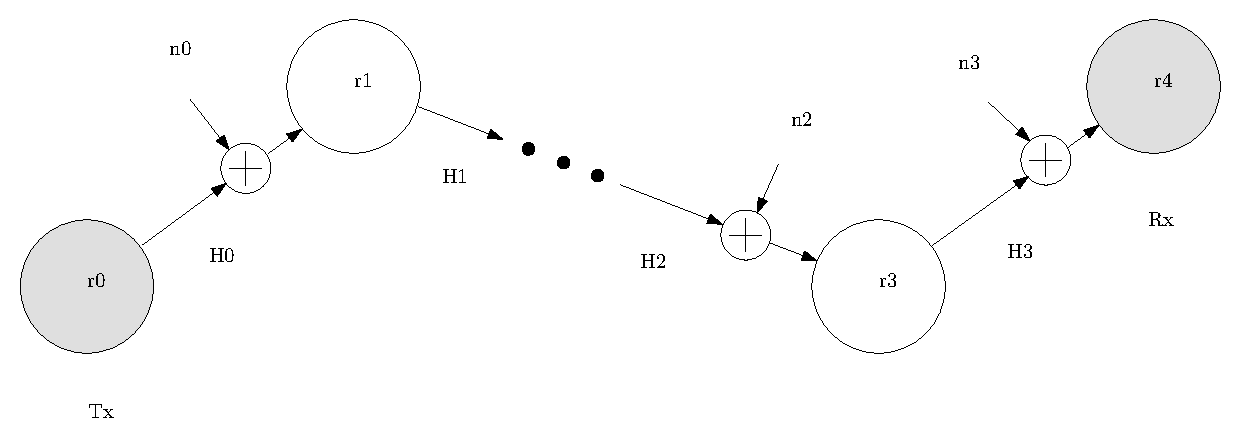
\includegraphics[width=2.5in]{sp_model.eps}
   \caption{Single Path Relay Network \label{fig:sp_sm} }
\end{figure}

In this section, we consider the single path relay network.  We first study the impact of power allocation to the mutual information for the amplify-and-forward and the decode-and-forward relay networks respectively and then present their WER performance from computer simulation.

\subsection{Amplify-and-Forward}
\label{sec:sp_af}
Figure \ref{fig:sp_sm} shows the single path
relay network. In the figure, $r_0$ is the transmitter, $r_{m+1}$
is the receiver, and $r_1, \ldots, r_m$ are $m$ relay nodes
connected in series forming a single path link between the
transmitter and receiver.  The relays perform amplify-and-forward
(AF) relaying. We assume that OFDM with $N$ subcarriers is used in
the system.  $h_k^{(0)}, \ldots, h_k^{(m)}$ are the complex subchannel gains at the $k^{\mbox{th}}$ subcarrier in the link, for $k = 1$ to $N$.   $n_k^{(0)}, \ldots, n_k^{(m)}$ are the corresponding noises, which are assumed to be mutually independent and circular symmetric complex Gaussians all with zero mean and variance $N_0 B / N$, where $N_0$ is the power spectral density of the underlying continuous time noise process and $B$ is the OFDM bandwidth of the system.  Let $p_k^{(0)} = P_{\mbox{tot}} / N$ be the transmit power on the $k^{\mbox{th}}$ subcarrier, where $P_{\mbox{tot}}$ is the net transmitter power and $\sqrt{p_k^{(l)}}$ be the amplifying gain used in the amplify-and-forward algorithm at the $l^{\mbox{th}}$ relay, for $l=1$ to $m$.  The $k^{\mbox{th}}$ receive symbol at $r_l$ is amplified by $\sqrt{p_k^{(l)}}$ before it is forwarded to the next node.  Let $x_k^{(0)}$ be the $k^{\mbox{th}}$ transmit symbol with zero mean and unit variance, $y_k$ be the $k^{\mbox{th}}$ receive symbol at the receiver, and $x_k^{(l)}$ be the $k^{\mbox{th}}$ receive symbol at the $l^{\mbox{th}}$ relay.  Note that $x_k^{(l)}$ is also the $k^{\mbox{th}}$ transmit symbol at the $l^{\mbox{th}}$ relay.

Using Figure \ref{fig:sp_sm}, the input-output relation at the $l^{\mbox{th}}$ relay is
\begin{eqnarray}
x_k^{(l)} = \left( \prod_{i=0}^{l-1} h_k^{(i)} \sqrt{p_k^{(i)}}
\right) x_k^{(0)} + \hspace{1.35in} \nonumber \\
\hspace{1.35in} \sum_{j=0}^{l-1} \left( \prod_{i=j+1}^{l-1}
h_k^{(i)} \sqrt{p_k^{(i)}} \right) n_k^{(j)} .
\label{eqn:sp_af_inout_relay_closed}
\end{eqnarray}
%\begin{eqnarray}
%x_k^{(l)} = \left( \prod_{i=0}^{l-1} h_k^{(i)} \sqrt{p_k^{(i)}}
%\right) x_k^{(0)} +  \sum_{j=0}^{l-1} \left( \prod_{i=j+1}^{l-1}
%h_k^{(i)} \sqrt{p_k^{(i)}} \right) n_k^{(j)} .
%\label{eqn:sp_af_inout_relay_closed}
%\end{eqnarray}
The input-output relation at the receiver is
\begin{eqnarray}
y_k = \left( \prod_{i=0}^m h_k^{(i)} \sqrt{p_k^{(i)}} \right)
x_k^{(0)} + \hspace{1.35in} \nonumber \\
\hspace{1.35in} \sum_{j=0}^m \left( \prod_{i=j+1}^m h_k^{(i)}
\sqrt{p_k^{(i)}} \right) n_k^{(j)}.
\label{eqn:sp_af_inout}
\end{eqnarray}
%\begin{eqnarray}
%y_k = \left( \prod_{i=0}^m h_k^{(i)} \sqrt{p_k^{(i)}} \right)
%x_k^{(0)} + \sum_{j=0}^m \left( \prod_{i=j+1}^m h_k^{(i)}
%\sqrt{p_k^{(i)}} \right) n_k^{(j)}.
%\label{eqn:sp_af_inout}
%\end{eqnarray}
Denote
%\begin{eqnarray}
%h_k = \displaystyle\prod_{i=0}^m  h_k^{(i)} \sqrt{p_k^{(i)}}
%\mbox{,} & \gamma_k^{(j)} = \displaystyle\prod_{i=j+1}^m h_k^{(i)}
%\sqrt{p_k^{(i)}}, \hspace{.3cm} \mbox{and} & w_k = \sum_{l=0}^{m}\gamma_k^{(l)}n_k^{(l)}
%\label{eqn:sp_af_hk_gammak_wk}
%\end{eqnarray}
\begin{eqnarray}
h_k = \displaystyle\prod_{i=0}^m  h_k^{(i)} \sqrt{p_k^{(i)}}
\mbox{,} & \gamma_k^{(j)} = \displaystyle\prod_{i=j+1}^m h_k^{(i)}
\sqrt{p_k^{(i)}},
\label{eqn:sp_af_hk_gammak}
\end{eqnarray}
and
\begin{eqnarray}
w_k = \sum_{l=0}^{m}\gamma_k^{(l)}n_k^{(l)}.
\label{eqn:sp_af_wk}
\end{eqnarray}
Then, (\ref{eqn:sp_af_inout}) can be written as
\begin{eqnarray}
y_k = h_k x_k + w_k \mbox{.} \label{eqn:sp_af_inout_terse}
\end{eqnarray}
Now, consider the variance of $w_k$.  Using
(\ref{eqn:sp_af_hk_gammak}) and (\ref{eqn:sp_af_wk}), we have
\begin{eqnarray}
R_{w_kw_k} & = & E \left[ w_k w_k^* \right] \nonumber \\  & = &
\frac{N_0B}{N} \sum_{j=0}^{m} \left( \prod_{i=j+1}^mb_k^{(i)}
p_k^{(i)}  \right) , \label{eqn:sp_af_Rwkwk}
\end{eqnarray}
where $E\left[ \cdot \right]$ is the expectation operator,
$\left(\cdot\right)^*$ is the complex conjugate operator for a
scalar, and $b_k^{(i)} = \left| h_k^{(i)} \right|^2$, for $i=0$ to
$m$.  $R_{w_kw_k}$ is positive for a nonzero $N_0$.  We define a
normalized version of the system in (\ref{eqn:sp_af_inout_terse})
\begin{eqnarray}
\tilde{y}_k = \tilde{h}_k x_k + \tilde{w}_k,
\end{eqnarray}
where $\tilde{y}_k = y_k / \sqrt{R_{w_kw_k}}$, $\tilde{h}_k = h_k
/ \sqrt{R_{w_kw_k}}$, and $\tilde{w}_k = w_k / \sqrt{R_{w_kw_k}}$.
The variances of $\tilde{w}_k$ and $\tilde{y}_k$ are
\begin{eqnarray}
E \left[ \tilde{w}_k \tilde{w}_k^* \right] = 1 \mbox{,}
\end{eqnarray}
and
\begin{eqnarray}
E \left[ \tilde{y}_k \tilde{y}_k^* \right] = \frac{1}{R_{w_kw_k}}
\left( \prod_{i=0}^m b_k^{(i)} p_k^{(i)} \right) + 1
\label{eqn:sp_af_yk_tilde_var} \mbox{,}
\end{eqnarray}
respectively.  The cross terms do not appear in
(\ref{eqn:sp_af_yk_tilde_var}) because $\tilde{h_k}$,
$\tilde{w_k}$, and $x_k$ are mutually independent.  Note that the
normalized system has unit variance noise.

\subsubsection{Mutual Information}
To derive the mutual information, note that the differential
entropy of a circular symmetric complex Gaussian vector,
$\mathbf{v}$, with covariance matrix, $\mathbf{K}$, is
$h\left(\mathbf{v}\right) = \log_2 \det \left( \pi e \mathbf{K}
\right)$ \cite{article:Telatar01}.  When the circular symmetric
complex Gaussian is a scalar, $v$, the differential entropy is
$h\left(v\right) = \log_2 \left( \pi e \sigma_v^2 \right)$, where
$\sigma_v^2$ is the variance of $v$.  Let $\mathcal{I}_k$ be the
mutual information between the transmitter and receiver on the
$k^{\mbox{th}}$ subcarrier
\begin{eqnarray}
\mathcal{I}_k & = & h\left( \tilde{y}_k \right) - h \left( \tilde{w}_k \right) \nonumber \\
& = & \log_2 \left[ \frac{1}{R_{w_kw_k}} \left( \prod_{i=0}^m
b_k^{(i)} p_k^{(i)} \right) + 1 \right]. \label{eqn:sp_af_Ik}
\end{eqnarray}
The total mutual information between the transmitter and receiver,
$\mathcal{I}$, is the sum of all $\mathcal{I}_k$ divided by $N$.
That is, after substituting (\ref{eqn:sp_af_Rwkwk}) into
(\ref{eqn:sp_af_Ik}), we have
\begin{eqnarray}
\mathcal{I} = \hspace{2.8in} \nonumber \\
\frac{1}{N} \sum_{k=1}^N \log_2 \left( 1 + \mbox{SNR} \left[
\frac{b_k^{(0)}\left( \prod_{i=1}^m b_k^{(i)} p_k^{(i)} \right)}
{\sum_{j=0}^m \left( \prod_{i=j+1}^m b_k^{(i)} p_k^{(i)} \right)
}\right]
 \right),
\label{eqn:sp_af_I}
\end{eqnarray}
%\begin{eqnarray}
%\mathcal{I} =
%\frac{1}{N} \sum_{k=1}^N \log_2 \left( 1 + \mbox{SNR} \left[
%\frac{b_k^{(0)}\left( \prod_{i=1}^m b_k^{(i)} p_k^{(i)} \right)}
%{\sum_{j=0}^m \left( \prod_{i=j+1}^m b_k^{(i)} p_k^{(i)} \right)
%}\right]
% \right),
%\label{eqn:sp_af_I}
%\end{eqnarray}
where $\mbox{SNR} = P_{\mbox{tot}} / N_0 B$.

\subsubsection{Relay Power Allocation}
We assume that the net transmit power at the transmitter and at
each each relay is $P_{\mbox{tot}}$, that is,
\begin{eqnarray}
\sum_{k=1}^N E \left\{ \left| \sqrt{p_k^{(l)}} x_k^{(l)} \right| ^2 \right\} = P_{\mbox{tot}}.
\label{eqn:sp_af_powerconstraint_simple}
\end{eqnarray}
At the transmitter, we assume a uniform power distribution, that is, $p_k^{(0)} = P_{\mbox{tot}}/N$.  To derive the power constraint at each relay, substitute (\ref{eqn:sp_af_inout_relay_closed}) into (\ref{eqn:sp_af_powerconstraint_simple}) to arrive at
\begin{eqnarray}
\sum_{k=1}^N \frac{ p_k^{(l)}}{N} \left[
b_k^{(0)} \left( \prod_{i=1}^{l-1}  b_k^{(i)}p_k^{(i)} \right) +
\frac{1}{\mbox{SNR}} \sum_{j=0}^{l-1} \prod_{i=j+1}^{l-1}  b_k^{(i)}p_k^{(i)} \right] \nonumber \\
=1. \label{eqn:sp_af_powerconstraint}
\end{eqnarray}
%\begin{eqnarray}
%\sum_{k=1}^N \frac{ p_k^{(l)}}{N} \left[
%b_k^{(0)} \left( \prod_{i=1}^{l-1}  b_k^{(i)}p_k^{(i)} \right) +
%\frac{1}{\mbox{SNR}} \sum_{j=0}^{l-1} \prod_{i=j+1}^{l-1}  b_k^{(i)}p_k^{(i)} \right] =1. \label{eqn:sp_af_powerconstraint}
%\end{eqnarray}
Note that (\ref{eqn:sp_af_powerconstraint}) is defined
recursively.  The power constraint for $p_k^{(l)}$ depends on
$p_k^{(1)}, \dots, p_k^{(l-1)}$.  $p_k^{(1)}$ is the base case in
the recursion, which follows from
(\ref{eqn:sp_af_powerconstraint}), when $l = 1$.

One power allocation at the $l^{\mbox{th}}$ relay is to set $p_k^{(l)}$ constant for all subcarriers.  This results in moving $p_k^{(l)}$ in (\ref{eqn:sp_af_powerconstraint}) out of the summation because it is no longer a function of $k$
\begin{eqnarray}
p_{k,ct}^{(l)} = p_{ct}^{(l)} =  \hspace{2.35in} \nonumber \\
\frac{ N \mbox{SNR} } { \displaystyle \sum_{k=1}^N \left[
\mbox{SNR} b_k^{(0)} \left( \displaystyle \prod_{i=1}^{l-1}
b_k^{(i)} p_{ct}^{(i)}\right) + \displaystyle \sum_{j=0}^{l-1}
\displaystyle \prod_{i=j+1}^{l-1} b_k^{(i)} p_{ct}^{(i)} \right]}.
\label{eqn:sp_af_ct_allocation}
\end{eqnarray}
%\begin{eqnarray}
%p_{k,ct}^{(l)} = p_{ct}^{(l)} = \frac{ N \mbox{SNR} } { \displaystyle \sum_{k=1}^N \left[
%\mbox{SNR} b_k^{(0)} \left( \displaystyle \prod_{i=1}^{l-1}
%b_k^{(i)} p_{ct}^{(i)}\right) + \displaystyle \sum_{j=0}^{l-1}
%\displaystyle \prod_{i=j+1}^{l-1} b_k^{(i)} p_{ct}^{(i)} \right]}.
%\label{eqn:sp_af_ct_allocation}
%\end{eqnarray}
We call this \emph{constant gain allocation} (CT).  This is in fact the amplify-and-forward scheme as defined in \cite{thesis:Laneman01}, where a receive symbol is multiplied by a constant gain to satisfy a power constraint.  In our context, this means that every subcarrier is multiplied by the same gain, $p_{ct}^{(l)}$.  Note that this
power allocation does not require each relay to have any channel
state information (CSI).  That is, we do not actually need to use
(\ref{eqn:sp_af_ct_allocation}).  We can use
(\ref{eqn:sp_af_powerconstraint_simple}) directly to solve for
$p_{ct}^{(l)}$.

A second power allocation is to choose $p_k^{(l)}$ such that every subcarrier transmits the same power at the $l^{\mbox{th}}$ relay.  That is, (\ref{eqn:sp_af_powerconstraint_simple}) becomes $E \left\{ \left| \sqrt{p_{k,eq}^{(l)}} x_k^{(l)} \right| ^2 \right\} = P_{\mbox{tot}}/N$, for $k = 1$ to $N$.  This is equivalent to setting every summand on the left hand side of (\ref{eqn:sp_af_powerconstraint}) to $1/N$.  We then have
\begin{eqnarray}
p_{k,eq}^{(l)} = \frac{\mbox{SNR}}
{\mbox{SNR} b_k^{(0)} \left( \displaystyle\prod_{i=1}^{l-1}b_k^{(i)} p_{k,eq}^{(i)} \right) + \displaystyle\sum_{j=0}^{l-1}
\prod_{i=j+1}^{l-1}  b_k^{(i)} p_{k,eq}^{(i)}} \mbox{.}
\label{}
\end{eqnarray}
We call this \emph{equal power allocation} (EQ).  Note that this power allocation does require each relay to have the CSI of its upstream channels.

\subsection{Decode-and-Forward}
In decode-and-forward (DF), each relay fully recovers the information bits (with possible errors) after receiving an OFDM symbol.  It then converts the information bits back into an OFDM symbol and then transmits it.  The transmitter and all the relays transmit with the same uniform power distribution.  That is,
\begin{eqnarray}
p_k^{(0)} = p_k^{(l)} = \frac{P_{\mbox{tot}}}{N}\mbox{,}
\end{eqnarray}
for $k = 1$ to $N$ and for $l = 1$ to $m$.

Let $x_k^{(0)}$ be the $k^{\mbox{th}}$ transmit symbol from the transmitter and  $x_k^{(l)}$ be the $k^{\mbox{th}}$ transmit symbol from the $l^{\mbox{th}}$ relay, all with with zero mean and unit variance.  Let $y_k^{(m+1)}$ be the $k^{\mbox{th}}$ receive symbol at the receiver and  $y_k^{(l)}$ be the $k^{\mbox{th}}$ receive symbol at the $l^{\mbox{th}}$ relay.  Using Figure \ref{fig:sp_sm}, the input-ouput relation at the $l^{\mbox{th}}$ relay is
\begin{eqnarray}
y_k^{(l)} = h_k^{(l-1)} \sqrt{\frac{P_{\mbox{tot}}}{N}} x_k^{(l-1)} + n_k^{(l-1)} \mbox{.}
\end{eqnarray}
The input-output relation at the receiver is
\begin{eqnarray}
y_k^{(m+1)} =h_k^{(m)}  \sqrt{\frac{P_{\mbox{tot}}}{N}} x_k^{(m)} + n_k^{(m)} \mbox{.}
\end{eqnarray}

\subsection{Simulations}
\label{sec:sp_sims}

\begin{figure*}
    \psfrag{WER}[Bc][tc][0.8]{WER}
    \psfrag{SNR}[tc][Bc][0.8]{SNR (dB)}
    \psfrag{hard-af-ct----}[cl][cl][0.5]{hard, AF, CT}
    \psfrag{hard-af-eq----}[cl][cl][0.5]{hard, AF, EQ}
    \psfrag{hard-df----}[cl][cl][0.5]{hard, DF}
    \psfrag{soft-af-ct----}[cl][cl][0.5]{soft, AF, CT}
    \psfrag{soft-af-eq----}[cl][cl][0.5]{soft, AF, EQ}
    \psfrag{soft-df----}[cl][cl][0.5]{soft, DF}

\centerline{
    \subfigure[m=2]{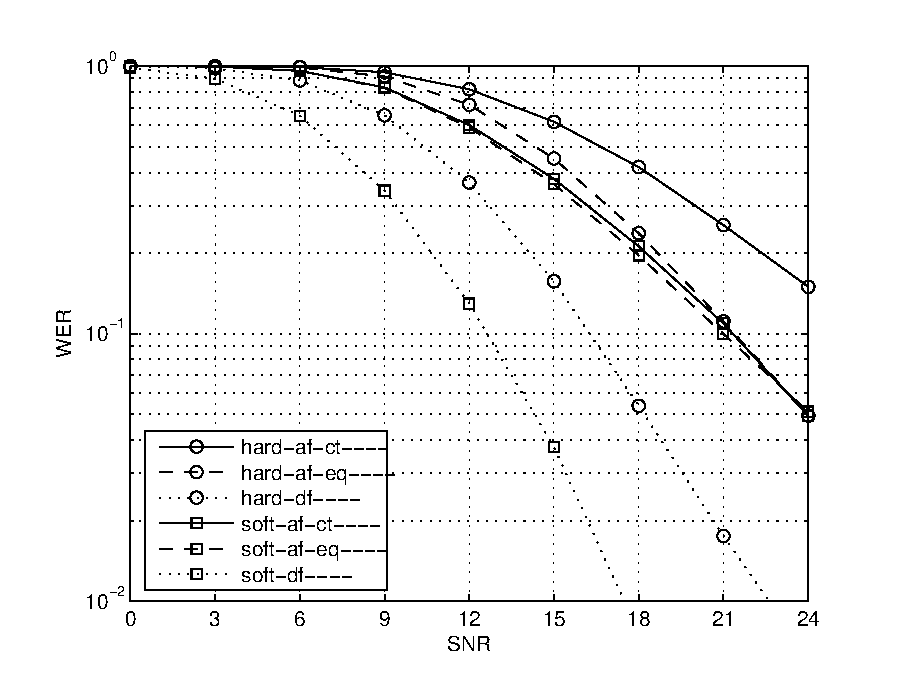
\includegraphics[width=3.25in]{sp_af_df_wer_m2_TU.eps} \label{}}
    \subfigure[m=4]{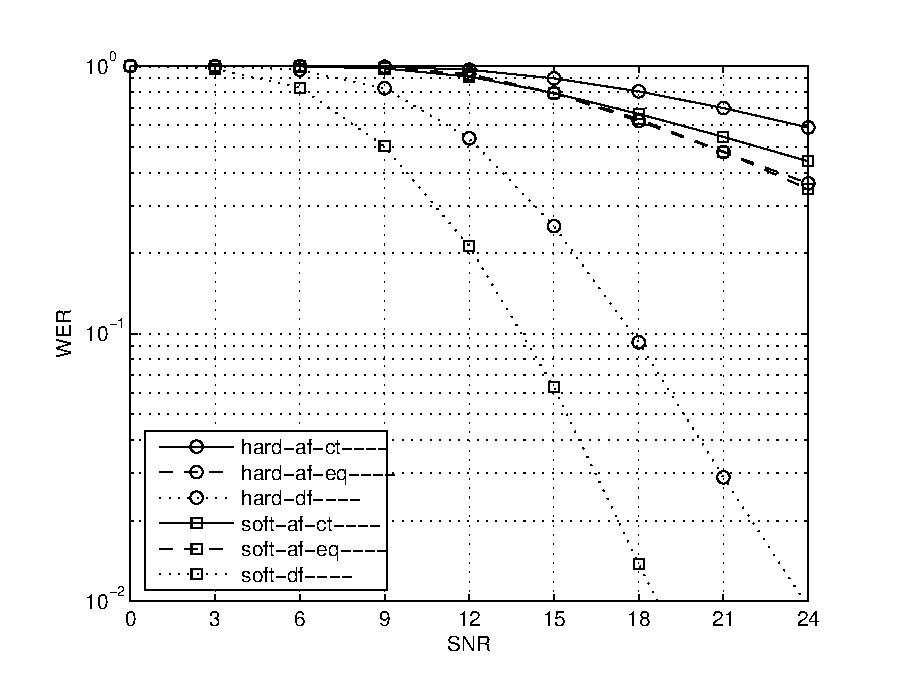
\includegraphics[width=3.25in]{sp_af_df_wer_m4_TU.eps} \label{}} \\
}
 \caption{WERs in a single path relay network
with TU channels using AF and DF.  $N = 128$.}
\label{fig:plots_sp}
\end{figure*}

We simulate WERs versus SNR for both the amplify-and-forward and decode-and-forward cases.  At the transmitter (and at the transmitter structure of a relay using decode-and-forward), each information word contains 83 bits.  We use a rate $\frac{1}{3}$ convolutional encoder with generator sequences $\left[1 1 1\right]$, $\left[1 1 1\right]$, and $\left[1 1 0\right]$ to encode the information word into a 255 bit codeword.  A zero bit is padded at the end to make 256 bits.  The bits are then interleaved and modulated onto $N = 128$ QPSK (quadrature phase shift keying) subcarriers to form one OFDM symbol.  At the receiver (and at the receiver structure of a relay using decode-and-forward), the codeword is recovered (with possible errors) using a matched filter and deinterleaving.  A Viterbi decoder is used to decode the codeword.  Both hard decisions and soft decisions are used.

We consider the $m = 2$ and $4$ relays cases.  We assume that all distances between any two adjacent transceiver nodes are the same.  Therefore, all path loss effects are normalized to 0 dB.  Shadowing is assumed to be log-normally distributed.  That is, the received power gain due to shadowing in dB is a zero-mean Gaussian with variance of 8 dB, which is typical for cellular land mobile applications \cite{book:Stuber01}.  We model frequency selective fading as Typical Urban (TU) channels \cite{book:Stuber01}.  We use an OFDM bandwidth of 800 kHz divided into $N = 128$ equal blocks.  Maintaining OFDM orthogonality, this translates into an OFDM symbol period of $T_s = 160 \:\mu$s.  The simulation results are shown in Figure \ref{fig:plots_sp}.

As shown in the plots, there are significant error rate
performance gains when using decode-and-forward instead of
amplify-and-forward.  The
gains are even larger when we increase the distance between the
transmitter and receiver (and thus, add more relays).  The
amplify-and-forward error rates suffer because more channel
distortion and noise enter the system.  The decode-and-forward
error rates suffer only slightly because noise and channel
distortion are eliminated at each relay.  This results in the
large performance gains for $m=4$.  In terms of power allocation
when using amplify-and-forward, CT is the preferable choice since
EQ requires CSI and only results in small performance gains over
CT.  As expected, soft decisions give better performance than hard
decisions in Viterbi decoding.

\section{Multiple Path Relay Network}
\label{sec:mp}

\begin{figure}
  \centering
    \psfrag{r0}[cc][Bl][0.8]{$r_0$}
    \psfrag{r1}[cc][Bl][0.8]{$r_1$}
    \psfrag{r3}[cc][Bl][0.8]{$r_m$}
    \psfrag{r4}[cc][Bl][0.8]{$r_{m+1}$}
    \psfrag{n01}[cc][Bl][0.8]{$n_k^{(0|1)}$}
    \psfrag{n03}[cc][Bl][0.8]{$n_k^{(0|m)}$}
    \psfrag{n14}[cc][Bl][0.8]{$n_k^{(1|m+1)}$}
    \psfrag{n34}[cc][Bl][0.8]{$n_k^{(m|m+1)}$}
    \psfrag{H01}[cc][Bl][0.8]{$h_k^{(0|1)}$}
    \psfrag{H03}[cc][Bl][0.8]{$h_k^{(0|m)}$}
    \psfrag{H14}[cc][Bl][0.8]{$h_k^{(1|m+1)}$}
    \psfrag{H34}[cc][Bl][0.8]{$h_k^{(m|m+1)}$}
    \psfrag{Tx}[cr][Bl][0.9]{Transmitter}
    \psfrag{Rx}[cl][Bl][0.9]{Receiver}
    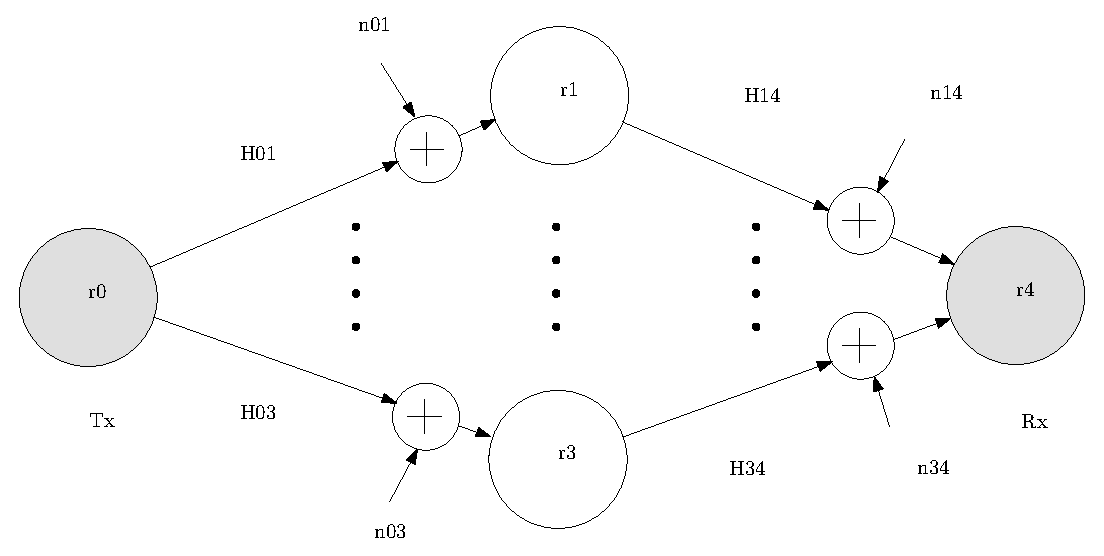
\includegraphics[width=2.5in]{mp_model.eps}
   \caption{Multiple Path Relay Network \label{fig:mp_sm} }
\end{figure}

In this section, we consider a multiple path relay network, following the same structure as Section \ref{sec:sp}.

\subsection{Amplify-and-Forward}
Figure \ref{fig:mp_sm} shows the multiple path relay network.  In the figure, $r_0$ is the transmitter, $r_{m+1}$ is the receiver, and $r_1, \ldots, r_m$ are $m$ relay nodes connected in parallel forming a multiple path link between the transmitter and receiver.  The relays perform amplify-and-forward (AF) relaying.  We assume that OFDM with $N$ subcarriers is used in the system.  $h_k^{(0|1)}, \ldots, h_k^{(0|m)}, h_k^{(1|m+1)}, \ldots, h_k^{(m|m+1)}$ are the complex subchannel gains at the $k^{\mbox{th}}$ subcarrier in the link, for $k = 1$ to $N$.   $n_k^{(0|1)}, \ldots, n_k^{(0|m)}, n_k^{(1|m+1)}, \ldots, n_k^{(m|m+1)}$ are the corresponding noises, which are assumed to be mutually independent, zero-mean, circular symmetric complex Gaussians all with variance $N_0 B / N$, where $N_0$ is the power spectral density of the underlying continuous time noise process and $B$ is the OFDM bandwidth of the system.  Let $p_k^{(0)} = P_{\mbox{tot}}/N$ be the transmitter power on the $k^{\mbox{th}}$ subcarrier, where $P_{\mbox{tot}}$ is the net transmitter power and $\sqrt{p_k^{(l)}}$ be the amplifying gain used in the amplify-and-forward algorithm at the $l^{\mbox{th}}$ relay, for $l=1$ to $m$.  The $k^{\mbox{th}}$ receive symbol at $r_l$ is amplified by $\sqrt{p_k^{(l)}}$ before it is forwarded to the next node.  Let $x_k$ be the $k^{\mbox{th}}$ transmit symbol with zero mean and unit variance and $y_k^{(l)}$  be the $k^{\mbox{th}}$ receive symbol from the $l^{\mbox{th}}$ path at the receiver.

Using Figure \ref{fig:mp_sm}, the input-output relation for the $l^{\mbox{th}}$ path is
\begin{eqnarray}
y_k^{(l)} = \left( h_k^{(0|l)} h_k^{(l|m+1)} \sqrt{p_k^{(0)}} \sqrt{p_k^{(l)}} \right) x_k
+ \hspace{.75in} \nonumber \\
\hspace{.75in} h_k^{(l|m+1)} \sqrt{p_k^{(l)}}  n_k^{(0|l)} +
n_k^{(l|m+1)}. \label{eqn:mp_af_inout}
\end{eqnarray}
%\begin{eqnarray}
%y_k^{(l)} = \left( h_k^{(0|l)} h_k^{(l|m+1)} \sqrt{p_k^{(0)}} \sqrt{p_k^{(l)}} \right) x_k
%+ h_k^{(l|m+1)} \sqrt{p_k^{(l)}}  n_k^{(0|l)} +
%n_k^{(l|m+1)}. \label{eqn:mp_af_inout}
%\end{eqnarray}
Denote
\begin{eqnarray}
\mathbf{y}_k = \left[
\begin{array}{ccc}
y_k^{(1)} & \cdots & y_k^{(m)}
\end{array} \right]^T,
\end{eqnarray}
\begin{eqnarray}
\mathbf{h}_k = \left[ \begin{array}{c} h_k^{(0|1)}h_k^{(1|m+1)}
\sqrt{p_k^{(0)}}
\sqrt{p_k^{(1)}} \\ \vdots  \\
h_k^{(0|m)}h_k^{(m|m+1)} \sqrt{p_k^{(0)}} \sqrt{p_k^{(m)}}
\end{array} \right], \label{eqn:mp_af_hk}
\end{eqnarray}
\begin{eqnarray}
\mathbf{\Gamma}_k = \hspace{2.8in} \nonumber \\
\left[
\begin{array}{ccccccc}
h_k^{(1|m+1)} \sqrt{p_k^{(1)}}&  & \textbf{\mbox{\huge{0}}} &   \\
 & \ddots & &  \textbf{\mbox{\huge{I}}}_{m \times m}    \\
\textbf{\mbox{\huge{0}}} &  &h_k^{(m|m+1)} \sqrt{p_k^{(m)}} &
\end{array}
\right] \mbox{,} \label{eqn:mp_af_Gammak}
\end{eqnarray}
%\begin{eqnarray}
%\mathbf{\Gamma}_k =
%\left[
%\begin{array}{ccccccc}
%h_k^{(1|m+1)} \sqrt{p_k^{(1)}}&  & \textbf{\mbox{\huge{0}}} &   \\
% & \ddots & &  \textbf{\mbox{\huge{I}}}_{m \times m}    \\
%\textbf{\mbox{\huge{0}}} &  &h_k^{(m|m+1)} \sqrt{p_k^{(m)}} &
%\end{array}
%\right] \mbox{,} \label{eqn:mp_af_Gammak}
%\end{eqnarray}
%\begin{eqnarray}
%\mathbf{n}_k = \left[
%\begin{array}{c}
%n_k^{(0|1)} \\ \vdots  \\ n_k^{(0|m)}
%\\ n_k^{(1|m+1)} \\  \vdots  \\ n_k^{(m|m+1)}
%\end{array}  \right] \mbox{,}
%\label{eqn:mp_af_nk}
%\end{eqnarray}
%\begin{eqnarray}
%\mathbf{n}_k = \left[
%\begin{array}{cccccc}
%n_k^{(0|1)} & \ldots  & n_k^{(0|m)} &  n_k^{(1|m+1)} &  \ldots  & n_k^{(m|m+1)}
%\end{array}  \right]^T \mbox{,}
%\label{eqn:mp_af_nk}
%\end{eqnarray}
\begin{eqnarray}
\mathbf{n}_k = \left[
\begin{array}{c}
n_k^{(0|1)} \\ \vdots  \\ n_k^{(0|m)} \\  n_k^{(1|m+1)} \\  \vdots  \\ n_k^{(m|m+1)}
\end{array}  \right] \mbox{,}
\label{eqn:mp_af_nk}
\end{eqnarray}
and
\begin{eqnarray}
\mathbf{w}_k = \mathbf{\Gamma}_k \mathbf{n}_k \mbox{.}
\label{eqn:mp_af_wk}
\end{eqnarray}
Then (\ref{eqn:mp_af_inout}), for all $l = 1$ to $m$, can be
written as
\begin{eqnarray}
\mathbf{y}_k = \mathbf{h}_k x_k + \mathbf{w}_k \mbox{.}
\label{eqn:mp_af_inout_terse}
\end{eqnarray}
The large boldface zeros in (\ref{eqn:mp_af_Gammak}) represent
zero values in the off diagonal entries in the left $m \times m$
submatrix of $\mathbf{\Gamma}_k$.

Now, consider the covariance of $\mathbf{w}_k$.  Using
(\ref{eqn:mp_af_hk}) to (\ref{eqn:mp_af_wk}), we have
\begin{eqnarray}
R_{\mathbf{w}_k\mathbf{w}_k} = \hspace{2.5 in} \nonumber \\
\frac{N_0B}{N} \left[
\begin{array}{ccc}
b_k^{(1|m+1)} p_k^{(1)}  + 1 & & \textbf{\mbox{\huge{0}}} \\
 & \ddots & \\
\textbf{\mbox{\huge{0}}}  & &  b_k^{(m|m+1)} p_k^{(m)} + 1
\end{array} \right],
\label{eqn:mp_af_Rwkwk}
\end{eqnarray}
where $b_k^{(i|j)} = \left| h_k^{(i|j)} \right|^2$, for $i=0$ to
$m$, for $j=1$ to $m+1$, and $i \neq j$. Since the diagonal
entries of $R_{\mathbf{w}_k\mathbf{w}_k}$ are never zero,
$R_{\mathbf{w}_k\mathbf{w}_k}^{-1}$ and
$R_{\mathbf{w}_k\mathbf{w}_k}^{-\frac{1}{2}}$ are well defined,
where
$R_{\mathbf{w}_k\mathbf{w}_k}^{-\frac{1}{2}}R_{\mathbf{w}_k\mathbf{w}_k}^{-\frac{1}{2}}
= R_{\mathbf{w}_k\mathbf{w}_k}^{-1}$. Also, if we define
$R_{\mathbf{w}_k\mathbf{w}_k}$ as
$R_{\mathbf{w}_k\mathbf{w}_k}^{\frac{1}{2}}
R_{\mathbf{w}_k\mathbf{w}_k}^{\frac{1}{2}}
=R_{\mathbf{w}_k\mathbf{w}_k}$, then
$R_{\mathbf{w}_k\mathbf{w}_k}^{-\frac{1}{2}}R_{\mathbf{w}_k\mathbf{w}_k}^{\frac{1}{2}}
=
R_{\mathbf{w}_k\mathbf{w}_k}^{\frac{1}{2}}R_{\mathbf{w}_k\mathbf{w}_k}^{-\frac{1}{2}}
= \mathbf{I}$. We define a normalized version of the system in
(\ref{eqn:mp_af_inout_terse})
\begin{eqnarray}
\tilde{\mathbf{y}}_k = \tilde{\mathbf{h}}_k x_k +
\tilde{\mathbf{w}}_k,
\end{eqnarray}
where $\tilde{\mathbf{y}}_k =
R_{\mathbf{w}_k\mathbf{w}_k}^{-\frac{1}{2}} \mathbf{y}_k$,
$\tilde{\mathbf{h}}_k =R_{\mathbf{w}_k\mathbf{w}_k}^{-\frac{1}{2}}
\mathbf{h}_k$, and $\tilde{\mathbf{w}}_k =
R_{\mathbf{w}_k\mathbf{w}_k}^{-\frac{1}{2}} \mathbf{w}_k$.  The
covariance matrices of $\tilde{\mathbf{w}}_k$ and
$\tilde{\mathbf{y}}_k$ are
\begin{eqnarray}
E \left[ \tilde{\mathbf{w}}_k \tilde{\mathbf{w}}_k^H \right]
 = \mathbf{I}
\end{eqnarray}
and
\begin{eqnarray}
E \left[ \tilde{\mathbf{y}}_k \tilde{\mathbf{y}}_k^H
\right]=\tilde{\mathbf{h}}_k \tilde{\mathbf{h}}_k^H + \mathbf{I},
\label{eqn:mp_af_yk_tilde_covar}
\end{eqnarray}
respectively.  The cross terms do not appear in
(\ref{eqn:mp_af_yk_tilde_covar}) because $\tilde{\mathbf{h}_k}$,
$\tilde{\mathbf{w}_k}$ and $x_k$ are mutually independent.  Note
that the normalized system has identity covariance noise.

\subsubsection{Mutual Information}
Let $\mathcal{I}_k$ be the mutual information between the
transmitter and receiver on the $k^{\mbox{th}}$ subcarrier
\begin{eqnarray}
\mathcal{I}_k & = & h\left( \tilde{\mathbf{y}}_k \right) - h \left( \tilde{\mathbf{w}}_k \right) \nonumber \\
& = & \log_2 \left( 1 + \mathbf{h}_k^H
R_{\mathbf{w}_k\mathbf{w}_k}^{-1} \mathbf{h}_k \right).
\label{eqn:mp_af_Ik}
\end{eqnarray}
The total mutual information between the transmitter and receiver,
$\mathcal{I}$, is the sum of all $\mathcal{I}_k$ divided by $N$.
That is, after substituting (\ref{eqn:mp_af_hk}) and
(\ref{eqn:mp_af_Rwkwk}) into (\ref{eqn:mp_af_Ik}), we have
%\begin{eqnarray}
%\mathcal{I} = \hspace{2.85in} \nonumber \\
% \frac{1}{N}  \sum_{k=1}^N \log_2 \left[ 1 +
%\mbox{SNR} \sum_{i=1}^m \left( \frac{b_k^{(0|i)}
%b_k^{(i|m+1)}p_k^{(i)}  }{ b_k^{(i|m+1)} p_k^{(i)}+1 }\right)
%\right], \label{eqn:mp_af_I}
%\end{eqnarray}
\begin{eqnarray}
\mathcal{I} =
 \frac{1}{N}  \sum_{k=1}^N \log_2 \left[ 1 +
\mbox{SNR} \sum_{i=1}^m \left( \frac{b_k^{(0|i)}
b_k^{(i|m+1)}p_k^{(i)}  }{ b_k^{(i|m+1)} p_k^{(i)}+1 }\right)
\right], \label{eqn:mp_af_I}
\end{eqnarray}
\subsubsection{Relay Power Allocation}
We assume that the net transmit power at the transmitter and at
each each relay is $P_{\mbox{tot}}$, as in
(\ref{eqn:sp_af_powerconstraint_simple}).  At the transmitter, we
assume a uniform power distribution, that is, $p_k^{(0)} =
P_{\mbox{tot}}/N$.  To derive the power constraint at each relay
and thus, possible power allocations, we use a derivation similar
to the one in Section \ref{sec:sp_af} to arrive at
\begin{eqnarray}
\sum_{k=1}^N \frac{ p_k^{(l)}}{N} \left(
b_k^{(0|l)} +
\frac{1}{\mbox{SNR}} \right) =1.
\label{eqn:mp_af_powerconstraint}
\end{eqnarray}

\emph{Constant gain allocation} (CT) in this case is
\begin{eqnarray}
p_{k,ct}^{(l)} = p_{ct}^{(l)} =
 \frac{N \mbox{SNR}}
{\displaystyle \sum_{k=1}^N \left( \mbox{SNR} b_k^{(0)} + 1 \right)
} \mbox{.}
\end{eqnarray}
Again, this power allocation does not require each relay to have
any channel state information (CSI).  The $l^{\mbox{th}}$ relay
only has to multiply its entire OFDM receive symbol by a constant,
$\sqrt{p_{ct}^{(l)}}$, such that the total transmit power is
$P_{\mbox{tot}}$, similar to constant gain allocation in Section
\ref{sec:sp_af}.

\emph{Equal power allocation} (EQ) in this case is
\begin{eqnarray}
p_{k,eq}^{(l)} =  \frac{ \mbox{SNR}}
{\displaystyle  \mbox{SNR} b_k^{(0|l)} + 1} \mbox{.}
\end{eqnarray}
Note that this power allocation does require each relay to have the CSI of its upstream channel.

\subsection{Decode-and-Forward}
In decode-and-forward (DF), each relay fully recovers the information bits (with possible errors) after receiving an OFDM symbol.  It then converts the information bits back into an OFDM symbol and then transmits it.  The transmitter and all the relays transmit with the same uniform power distribution.  That is,
\begin{eqnarray}
p_k^{(0)} = p_k^{(l)} = \frac{P_{\mbox{tot}}}{N}\mbox{,}
\end{eqnarray}
for $k = 1$ to $N$ and for $l = 1$ to $m$.

Let $x_k^{(0)}$ be the $k^{\mbox{th}}$ transmit symbol from the transmitter and  $x_k^{(l)}$ be the $k^{\mbox{th}}$ transmit symbol from the $l^{\mbox{th}}$ relay, all with with zero mean and unit variance.  Let $y_k^{(m+1)}$ be the $k^{\mbox{th}}$ receive symbol at the receiver and  $y_k^{(l)}$ be the $k^{\mbox{th}}$ receive symbol at the $l^{\mbox{th}}$ relay.  Using Figure \ref{fig:mp_sm}, the input-ouput relation at the $l^{\mbox{th}}$ relay is
\begin{eqnarray}
y_k^{(l)} = h_k^{(0|l)} \sqrt{\frac{P_{\mbox{tot}}}{N}} x_k^{(0)} + n_k^{(0|l)} \mbox{.}
\end{eqnarray}
The input-output relation at the receiver is
\begin{eqnarray}
y_k^{(m+1)} = \sum_{i=1}^m\left( h_k^{(i|m+1)}  \sqrt{\frac{P_{\mbox{tot}}}{N}} x_k^{(i)} + n_k^{(i|m+1)} \right)\mbox{.}
\end{eqnarray}
Note that in this situation, there are $m$ (modified in general) copies of the original $k^{\mbox{th}}$ transmit symbol $x_k^{(0)}$, namely, $x_k^{(1)}, \ldots, x_k^{(m)}$.  Therefore, the receiver has to assume (incorrectly in general) that all $m$ relays perform perfect recovery of the information bits so that $x_k^{(l)}$ = $x_k^{(0)}$.  That is, the receiver assumes the $k^{\mbox{th}}$ receive symbol is
\begin{eqnarray}
y_k^{(m+1)} = \left( \sum_{i=1}^m h_k^{(i|m+1)}
\sqrt{\frac{P_{\mbox{tot}}}{N}} \right) x_k^{(0)} + \sum_{i=1}^m
n_k^{(i|m+1)} \mbox{.}
\end{eqnarray}
This allows the receiver to use a filter that is matched to $\displaystyle \sum_{i=1}^m h_k^{(i|m+1)}$.

\subsection{Simulations}

\begin{figure*}
    \psfrag{WER}[Bc][tc][0.8]{WER}
    \psfrag{SNR}[tc][Bc][0.8]{SNR (dB)}
    \psfrag{hard-af-ct----}[cl][cl][0.5]{hard, AF, CT}
    \psfrag{hard-af-eq----}[cl][cl][0.5]{hard, AF, EQ}
    \psfrag{hard-df----}[cl][cl][0.5]{hard, DF}
    \psfrag{soft-af-ct----}[cl][cl][0.5]{soft, AF, CT}
    \psfrag{soft-af-eq----}[cl][cl][0.5]{soft, AF, EQ}
    \psfrag{soft-df----}[cl][cl][0.5]{soft, DF}

\centerline{
    \subfigure[m=2]{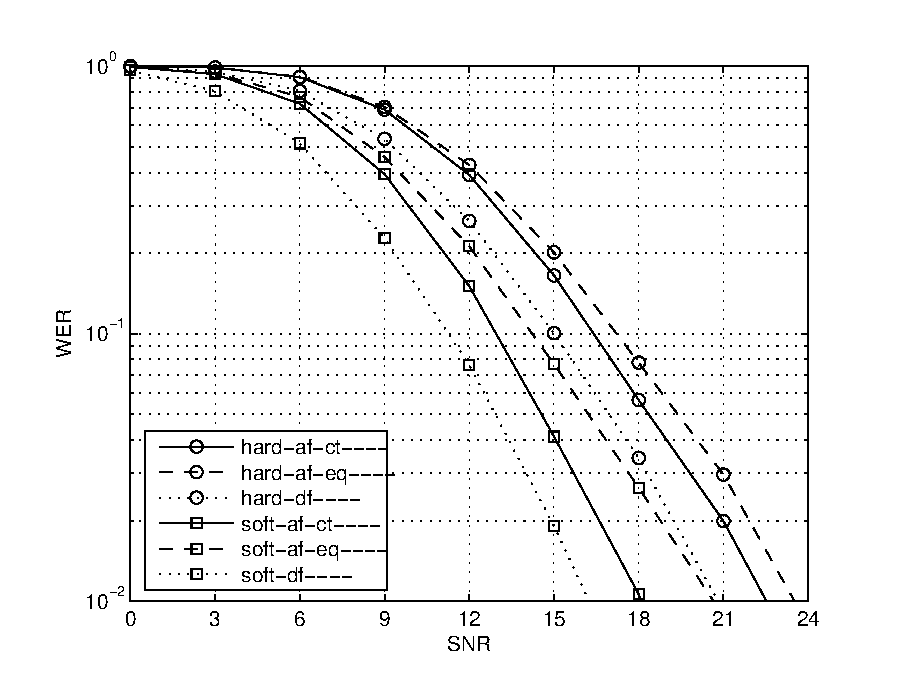
\includegraphics[width=3.25in]{mp_af_df_wer_m2_TU.eps} \label{}}
    \subfigure[m=4]{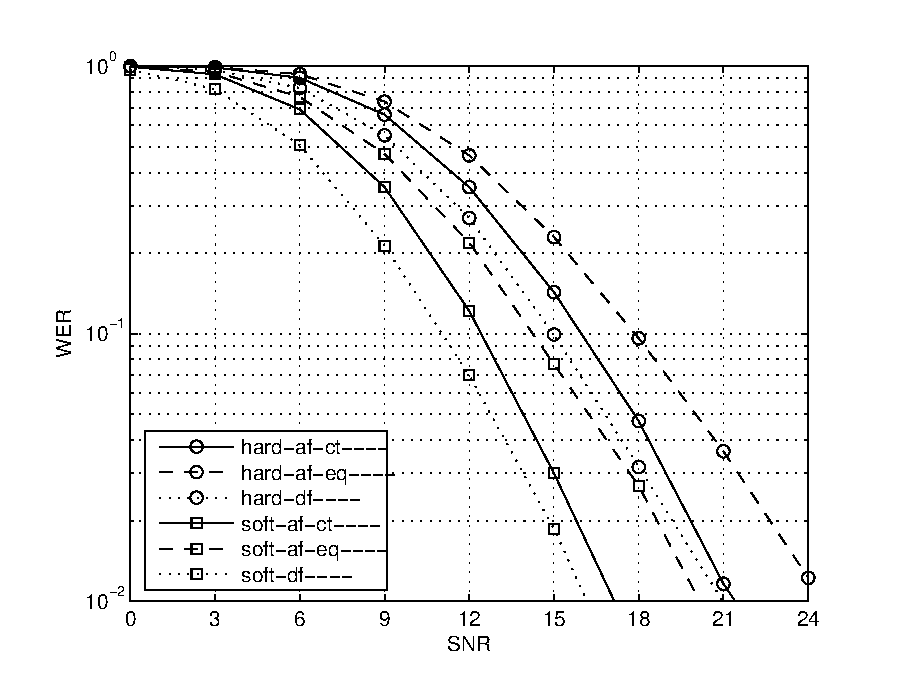
\includegraphics[width=3.25in]{mp_af_df_wer_m4_TU.eps} \label{}} \\
} \caption{WERs in a multiple path relay network
with TU channels using AF and DF.  $N = 128$.}
\label{fig:plots_mp}
\end{figure*}

We simulate WERs versus SNR for both the amplify-and-forward and decode-and-forward cases.  We use exactly the same configuration in Section \ref{sec:sp_sims}.  The simulation results are shown in Figure \ref{fig:plots_mp}.

The performance gains
resulting from using decode-and-forward instead of
amplify-and-forward diminish as we add more paths between the
transmitter and receiver (and thus, add more relays). This is
because for $m=4$ relays and thus, for 4 paths, the system is
already resistant to noise and channel distortion.  Therefore,
decode-and-forward cannot provide any more significant improvement
over amplify-and-forward.  In such a situation,
amplify-and-forward might be a more attractive choice due to its
lower complexity.  In terms of power allocation when using
amplify-and-forward, CT is the preferable choice because it gives
better performance than EQ and does not require CSI.  As expected, soft decisions give better performance than hard
decisions in Viterbi decoding.


\section{Conlcusions}
\label{sec:conclusions}

In this paper, we exploit cooperative relays by studying two subcarrier power allocation schemes as well as the system mutual information in OFDM-based wireless networks.  WER simulations indicate that the decode-and-forward relay algorithm provides better performance than that of amplify-and-forward in a single path relay network because the former is able to eliminate channel noise at each relay.  For the multiple path relay network, however, the network structure is already resistant to noise and channel distortion, and amplify-and-forward is more attractive due to its lower complexity.

Future research includes investigating additional relay algorithms, such as hybrid schemes.  For example, depending on the channel conditions, a relay can amplify-and-forward, decode-and-forward, or even just discard subcarrier symbols.  This in turn leads to more possibilities for relay power allocation.  In this paper, we only investigate the single path relay network and the multiple path relay network.  Other general relay networks need to be considered in the context of OFDM as well.  This will lend more insight into developing a general theoretical framework for OFDM in cooperative relay networks.

%\hspace{1cm}

\bibliographystyle{IEEEtran}
\bibliography{IEEEabrv,mybib}

\end{document}
